\documentclass[tikz,border=5pt]{standalone}
\usepackage{tikz}
\usetikzlibrary{arrows.meta}
\definecolor{nebula}{HTML}{6366F1}
\definecolor{spark}{HTML}{14B8A6}
\definecolor{ink}{HTML}{334155}
\begin{document}
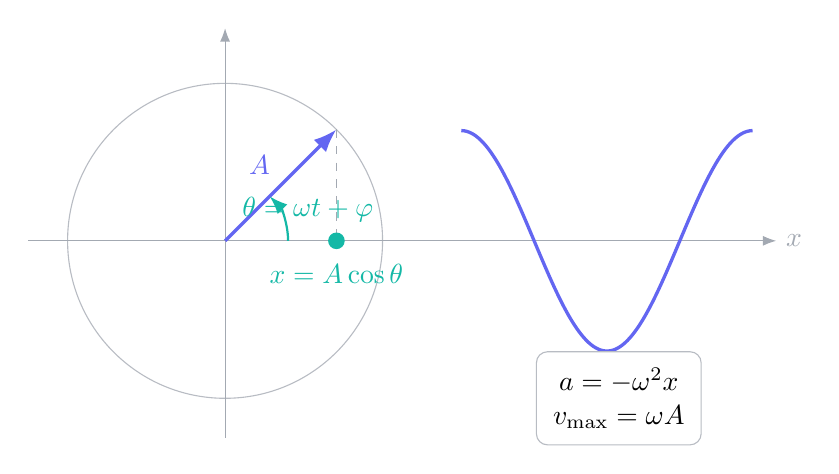
\begin{tikzpicture}[font=\sffamily,>=Latex]
  \draw[ink!35] (0,0) circle (2cm);
  \draw[->,ink!45] (-2.5,0)--(7,0) node[right] {$x$};
  \draw[->,ink!45] (0,-2.5)--(0,2.7);
  \coordinate (P) at (45:2);
  \draw[very thick,nebula,->] (0,0)--(P) node[midway,above left] {$A$};
  \draw[dashed,ink!45] (P)--({2*cos(45)},0);
  \fill[spark] ({2*cos(45)},0) circle (3pt) node[below=5pt] {$x=A\cos\theta$};
  \draw[->,spark,thick] (.8,0) arc[start angle=0,end angle=45,radius=.8];
  \node[spark] at (1.05,.4) {$\theta=\omega t+\varphi$};
  \draw[domain=3:6.7,samples=120,very thick,nebula] plot (\x,{1.4*cos(180*(\x-3)/1.85)});
  \node[align=center,draw=ink!35,rounded corners=4pt,fill=white,inner sep=6pt] at (5.0,-2.0) {$a=-\omega^2x$\\$v_{\max}=\omega A$};
\end{tikzpicture}
\end{document}
